
\documentclass[11pt,a4paper]{article}
\usepackage[utf8]{inputenc}
\usepackage[T1]{fontenc}
\usepackage{amsfonts}
\usepackage{amssymb}
\usepackage{mdframed}
\usepackage{tikz}
\usetikzlibrary{calc}
\usepackage{tkz-tab}
\usepackage{pgfplots}
\usepackage{xcolor}
\usepackage{fancyhdr}
\usepackage{lastpage}
\usepackage[fleqn]{amsmath}
\setlength{\mathindent}{0pt}

\newcommand{\pdt}{\mathbin{\vcenter{\hbox{\scalebox{0.6}{\textbullet}}}}}


% Spécifications du document
\newcommand{\doctitre}{Produit scalaire et applications} % Ex: Le second degré
\newcommand{\docniveau}{$1^{\text{re}}$ Spécialité mathématiques} % Ex: 1^{\text{re}}$ Spécialité mathématiques
\newcommand{\doctheme}{Géométrie} %Ex: Algèbre
\newcommand{\doctype}{Cours} % Ex: Démonstrations
\newcommand{\docshorttype}{Cours} % Démo

% Couleurs pour les graphiques
\definecolor{dark_green}{HTML}{008000}

% Paramètres du document
\RequirePackage{geometry}
\geometry{tmargin=1cm,bmargin=1.9cm,lmargin=1.9cm,rmargin=1.9cm}
\renewcommand{\familydefault}{\sfdefault}
\setlength{\parindent}{0pt}
\title{\doctitre}
\author{\docniveau \\ \doctheme\text{ - }\doctype}
\date{}
\fancypagestyle{custom}{
  \fancyhf{}
  \renewcommand{\headrulewidth}{0pt}
  \lfoot{\doctheme\text{ - }\docshorttype}
  \cfoot{\doctitre} % Change \titre to \doctitre
  \rfoot{\thepage/\pageref{LastPage}}
}

% Styles pour les mdframed
\mdfdefinestyle{definitionStyle}{
    leftline=true,
    rightline=false,
    topline=false,
    bottomline=false,
    linewidth=2pt,
    linecolor=black,
    innertopmargin=0pt,
    innerbottommargin=0pt,
    innerrightmargin=0pt,
    innerleftmargin=5pt,
}

\mdfdefinestyle{proprieteStyle}{
    linewidth=1pt,
    linecolor=black,
    innertopmargin=5pt,
    innerbottommargin=5pt,
    innerrightmargin=5pt,
    innerleftmargin=5pt,
}
% ----- DEBUT DU DOCUMENT -----
\begin{document}

% Style et numérotation
\maketitle
\pagestyle{custom}
\thispagestyle{custom}

\section*{I. Premières expressions du produit scalaire de deux vecteurs}

\subsection*{1. Formule avec le cosinus}

\begin{mdframed}[style=definitionStyle]
    \textbf{Définition \emph{(expression du produit scalaire n°1)} :} ~\\
    Si $\vec{u}$ et $\vec{v}$ sont deux vecteurs non nuls tels que $\vec{u}=\overrightarrow{AB}$ et
    $\vec{v}=\overrightarrow{AC}$, leurs produit scalaire est le nombre $\vec{u}\pdt\vec{v}= \| \vec{u} \| \times \|
        \vec{v} \| \times \cos{(u,v)} = AB \times AC \times \cos{(\widehat{BAC} )}$
\end{mdframed}

\textbf{Schéma :} ~\\
\begin{tikzpicture}[scale=1,>=stealth]

    \draw[] (-1,0) (5,0) ;
    \draw[] (0,-1) (0,4);

    % Définir les coordonnées des vecteurs u et v
    \coordinate (u) at (2,4);
    \coordinate (v) at (2.5,1);

    % Dessinez les vecteurs u et v
    \draw[->,thick,blue] (1,3) -- (u) node[midway,anchor=south east] {$\vec{u}$};
    \draw[->,thick,red] (1,2) -- (v) node[midway,anchor=north east] {$\vec{v}$};

    % Définir les coordonnées des points A et B
    \coordinate (A) at (3.5,2.5);
    \coordinate (B) at (4.5,3.5);
    \coordinate (C) at (5,1.5);

    % Marquer l'angle BAC
    \draw[black, line width=0.6pt] (3.8, 2.8) arc (60:-58:0.3) node[midway,anchor=west] {\scriptsize{$\widehat{BAC} $}};

    % Dessinez les vecteurs AB et AC
    \draw[->,thick,blue] (A) -- (B) node[midway,anchor=south west] {};
    \draw[->,thick,red] (A) -- (C) node[midway,anchor=north west] {};

    % Marquer les points A, B et C avec des croix plus petites et plus épaisses
    \draw[line width=0.6pt] (A) ++(-0.05,-0.05) -- ++(0.1,0.1) (A) ++(-0.05,0.05) -- ++(0.1,-0.1) node[anchor=south east] {\scriptsize{$A$}};
    \draw[line width=0.6pt] (B) ++(-0.05,-0.05) -- ++(0.1,0.1) (B) ++(-0.05,0.05) -- ++(0.1,-0.1) node[anchor=south west] {\scriptsize{$B$}};
    \draw[line width=0.6pt] (C) ++(-0.05,-0.05) -- ++(0.1,0.1) (C) ++(-0.05,0.05) -- ++(0.1,-0.1) node[anchor=south west] {\scriptsize{$C$}};
\end{tikzpicture}

\vspace{-45pt}
\textbf{Cas particulier \emph{(produit scalaire de deux vecteurs colinéaires)} :} ~\\

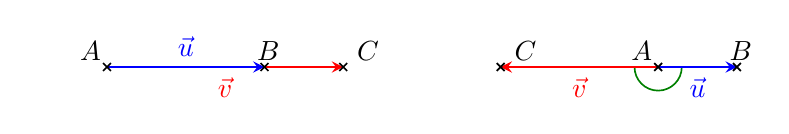
\begin{tikzpicture}[scale=1,>=stealth]

    \draw[] (-1,0) (5,0) ;

    % Définir les coordonnées des points A et B
    \coordinate (A1) at (0,0);
    \coordinate (B1) at (2,0);
    \coordinate (C1) at (3,0);

    \coordinate (C2) at (5,0);
    \coordinate (A2) at (7,0);
    \coordinate (B2) at (8,0);

    \draw[dark_green, line width=0.6pt] (7.3, 0) arc (0:-180:0.3) node[midway,anchor=west] {};

    % Dessinez les vecteurs AB et AC
    \draw[->,thick,red] (A1) -- (C1) node[midway,anchor=north] {$\vec{v}$};
    \draw[->,thick,blue] (A1) -- (B1) node[midway,anchor=south] {$\vec{u}$};
    \draw[->,thick,blue] (A2) -- (B2) node[midway,anchor=north] {$\vec{u}$};
    \draw[->,thick,red] (A2) -- (C2) node[midway,anchor=north] {$\vec{v}$};

    % Marquer les points A, B et C avec des croix plus petites et plus épaisses
    \draw[line width=0.6pt] (A1) ++(-0.05,-0.05) -- ++(0.1,0.1) (A1) ++(-0.05,0.05) -- ++(0.1,-0.1) node[anchor=south east] {$A$};
    \draw[line width=0.6pt] (B1) ++(-0.05,-0.05) -- ++(0.1,0.1) (B1) ++(-0.05,0.05) -- ++(0.1,-0.1) node[anchor=south] {$B$};
    \draw[line width=0.6pt] (C1) ++(-0.05,-0.05) -- ++(0.1,0.1) (C1) ++(-0.05,0.05) -- ++(0.1,-0.1) node[anchor=south west] {$C$};
    \draw[line width=0.6pt] (A2) ++(-0.05,-0.05) -- ++(0.1,0.1) (A2) ++(-0.05,0.05) -- ++(0.1,-0.1) node[anchor=south east] {$A$};
    \draw[line width=0.6pt] (B2) ++(-0.05,-0.05) -- ++(0.1,0.1) (B2) ++(-0.05,0.05) -- ++(0.1,-0.1) node[anchor=south] {$B$};
    \draw[line width=0.6pt] (C2) ++(-0.05,-0.05) -- ++(0.1,0.1) (C2) ++(-0.05,0.05) -- ++(0.1,-0.1) node[anchor=south west] {$C$};
\end{tikzpicture}

Si $C\in[AB)$, alors $\color{blue}\overrightarrow{AB}\color{black}\pdt\color{red}\overrightarrow{AC}\color{black}=\color{blue}AB\color{black}\times \color{red}AC\color{black}\times\cos{(\color{dark_green}0\color{black})}=\color{blue}AB\color{black}\times \color{red}AC$. \\
Si $C\not\in[AB)$, alors $\color{blue}\overrightarrow{AB}\color{black}\pdt\color{red}\overrightarrow{AC}\color{black}=\color{blue}AB\color{black}\times \color{red}AC\color{black}\times\cos{(\color{dark_green}180\color{black})}=\color{blue}-AB\color{black}\times \color{red}AC$. \\

\begin{mdframed}[style=definitionStyle]
    \textbf{Définition :} ~\\
    On appelle carré scalaire du vecteur $\vec{u}$ le nombre noté $\vec{u}^2$ et égal à $\vec{u}^2=\vec{u}\pdt\vec{u}= \| \vec{u} \| \times \| \vec{u}\| = \| \vec{u}\|^2$
\end{mdframed}

\subsection*{2. Formule du projeté orthogonal}

\begin{mdframed}[style=proprieteStyle]
    \textbf{Propriété \emph{(expression du produit scalaire n°2)} :} ~\\
    Soit $\overrightarrow{AB}$ et $\overrightarrow{AC}$ deux vecteurs du plan. $H$ est le projeté orthogonal du point
    $C$ sur la droite $AB$. \\
    Alors $\overrightarrow{AB}\pdt\overrightarrow{AC}=\overrightarrow{AB}\pdt\overrightarrow{AH}$
\end{mdframed}

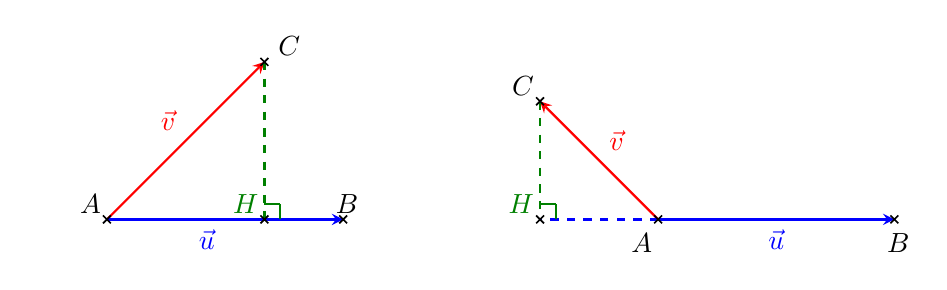
\begin{tikzpicture}[scale=1,>=stealth]

    \draw[] (-1,0) (5,0) ;

    % Définir les coordonnées des points A et B
    \coordinate (A1) at (0,0);
    \coordinate (B1) at (3,0);
    \coordinate (C1) at (2,2);
    \coordinate (H1) at (2,0);

    \coordinate (A2) at (7,0);
    \coordinate (B2) at (10,0);
    \coordinate (C2) at (5.5,1.5);
    \coordinate (H2) at (5.5,0);

    % Dessinez les vecteurs AB et AC
    \draw[->,thick,red] (A1) -- (C1) node[midway,anchor=south east] {$\vec{v}$};
    \draw[->,thick,blue] (A1) -- (B1) node[midway,anchor=north east] {$\vec{u}$};
    \draw[thick,dark_green, dashed] (C1) -- (H1) node[midway,anchor=north east] {};

    \draw[->,thick,blue] (A2) -- (B2) node[midway,anchor=north] {$\vec{u}$};
    \draw[->,thick,red] (A2) -- (C2) node[midway,anchor=south west] {$\vec{v}$};
    \draw[thick,dark_green, dashed] (C2) -- (H2) node[midway,anchor=north east] {};
    \draw[thick,blue, dashed] (A2) -- (H2) node[midway,anchor=north east] {};

    \draw[thick,dark_green] (2.2,0) -- (2.2,0.2) node[midway,anchor=north east] {};
    \draw[thick,dark_green] (2,0.2) -- (2.2,0.2) node[midway,anchor=north east] {};

    \draw[thick,dark_green] (5.7, 0) -- (5.7,0.2) node[midway,anchor=north east] {};
    \draw[thick,dark_green] (5.5, 0.2) -- (5.7,0.2) node[midway,anchor=north east] {};

    % Marquer les points A, B et C avec des croix plus petites et plus épaisses
    \draw[line width=0.6pt] (A1) ++(-0.05,-0.05) -- ++(0.1,0.1) (A1) ++(-0.05,0.05) -- ++(0.1,-0.1) node[anchor=south east] {$A$};
    \draw[line width=0.6pt] (B1) ++(-0.05,-0.05) -- ++(0.1,0.1) (B1) ++(-0.05,0.05) -- ++(0.1,-0.1) node[anchor=south] {$B$};
    \draw[line width=0.6pt] (C1) ++(-0.05,-0.05) -- ++(0.1,0.1) (C1) ++(-0.05,0.05) -- ++(0.1,-0.1) node[anchor=south west] {$C$};
    \draw[line width=0.6pt] (H1) ++(-0.05,-0.05) -- ++(0.1,0.1) (H1) ++(-0.05,0.05) -- ++(0.1,-0.1) node[anchor=south east] {$\color{dark_green}H$};

    \draw[line width=0.6pt] (A2) ++(-0.05,-0.05) -- ++(0.1,0.1) (A2) ++(-0.05,0.05) -- ++(0.1,-0.1) node[anchor=north east] {$A$};
    \draw[line width=0.6pt] (B2) ++(-0.05,-0.05) -- ++(0.1,0.1) (B2) ++(-0.05,0.05) -- ++(0.1,-0.1) node[anchor=north] {$B$};
    \draw[line width=0.6pt] (C2) ++(-0.05,-0.05) -- ++(0.1,0.1) (C2) ++(-0.05,0.05) -- ++(0.1,-0.1) node[anchor=south east] {$C$};
    \draw[line width=0.6pt] (H2) ++(-0.05,-0.05) -- ++(0.1,0.1) (H2) ++(-0.05,0.05) -- ++(0.1,-0.1) node[anchor=south east] {$\color{dark_green}H$};
\end{tikzpicture}

\newpage
\section*{II. Propriétés du produit scalaire}

\subsection*{1. Symétrie et bilinéarité}

\begin{mdframed}[style=proprieteStyle]
    \textbf{Propriétés :} ~\\
    Soit $\vec{u}$, $\vec{v}$ et $\vec{w}$ des vecteurs du plan et $k$ un réel.
    \vspace{-3pt}
    \begin{itemize}
        \item $\vec{u}\pdt\vec{v}=\vec{v}\pdt\vec{u}$ \quad \emph{(symétrie)}
        \item $\vec{u}\pdt(\vec{v}+\vec{w})=\vec{u}\pdt\vec{v}+\vec{u}\pdt\vec{w}$ \quad \emph{(bilinéarité)}
        \item $(k\vec{u})\pdt\vec{v}=\vec{u}\pdt(k\vec{v})=k(\vec{u}\pdt\vec{v})$ \quad \emph{(bilinéarité)}
    \end{itemize}
\end{mdframed}

\subsection*{2. Expression du produit scalaire dans un repère orthonormé}

\begin{mdframed}[style=proprieteStyle]
    \textbf{Propriété \emph{(expression du produit scalaire n°3)} :} ~\\
    Si $\vec{u}$ et $\vec{v}$ sont deux vecteurs de coordonnées respectives $\displaystyle \binom{x}{y}$ et $\displaystyle \binom{x'}{y'}$ dans un repère orthonormé. \\
    Alors $\vec{u}\pdt\vec{v}=xx'+yy'$
\end{mdframed}

\textbf{Remarque :} Dans un repère orthonormé, on a $\| \vec{u} \|^2=\vec{u}\pdt\vec{u}=x^2+y^2$. D'où $\| \vec{u} \|=\sqrt{x^2+y^2}$.

\subsection*{3. Identités remarquables avec le produit scalaire}

\begin{mdframed}[style=proprieteStyle]
    \textbf{Théorème \emph{(identités remarquables concernant le produit scalaire)} :}
    \begin{itemize}
        \item $(\vec{u}+\vec{v})^2=\|\vec{u}\|^2+2\vec{u}\pdt\vec{v}+\|\vec{v}\|^2$
        \item $(\vec{u}-\vec{v})^2=\|\vec{u}\|^2-2\vec{u}\pdt\vec{v}+\|\vec{v}\|^2$
        \item $(\vec{u}+\vec{v})\pdt(\vec{u}-\vec{v})=\|\vec{u}\|^2-\|\vec{v}\|^2$
    \end{itemize}
\end{mdframed}

\begin{mdframed}[style=proprieteStyle]
    \textbf{Conséquences \emph{(nouvelles expressions du produit scalaire)} :}
    \begin{itemize}
        \item $\vec{u}\pdt\vec{v}=\frac{1}{2}\left( \| \vec{u}+\vec{v} \|^2 - \|\vec{u}\|^2 - \|\vec{v}\|^2 \right)$ \quad \emph{(expression n°4)}
        \item $\vec{u}\pdt\vec{v}=\frac{1}{2}\left(\|\vec{u}\|^2 + \|\vec{v}\|^2 - \| \vec{u}-\vec{v} \|^2 \right)$ \quad \emph{(expression n°5)}
        \item $\vec{u}\pdt\vec{v}=\frac{1}{4}\left( \| \vec{u}+\vec{v} \|^2 - \| \vec{u}-\vec{v} \|^2 \right)$ \quad \emph{(expression n°6)}
    \end{itemize}
\end{mdframed}

\subsection*{4. Orthogonalité}

\begin{mdframed}[style=definitionStyle]
    \textbf{Définition :} ~\\
    On dit que les vecteurs $\overrightarrow{AB}$ et $\overrightarrow{CD}$ sont orthogonaux lorsque les droites $(AB)$ et $(CD)$ sont perpendiculaires.
\end{mdframed}

\begin{mdframed}[style=proprieteStyle]
    \textbf{Propriété :} ~\\
    Soit $\vec{u}$ et $\vec{v}$ deux vecteurs non nuls. \\
    Deux vecteurs $\vec{u}$ et $\vec{v}$ sont orthogonaux si et seulement si $\vec{u}\pdt\vec{v}=0$.
\end{mdframed}

\begin{mdframed}[style=proprieteStyle]
    \textbf{Propriété \emph{(critères d'orthogonalité dans un repère orthonormé)} :} ~\\
    Dans un repère orthonormé, les vecteurs $\displaystyle\vec{u}\binom{x}{y}$ et $\displaystyle\vec{v}\binom{x'}{y'}$ sont orthogonaux si et seulement si $xx'+yy'=0$.
\end{mdframed}

\newpage

\section*{III. Application du produit scalaire}

\subsection*{1. Théorème de la médiane}





\begin{minipage}{0.3\textwidth}
    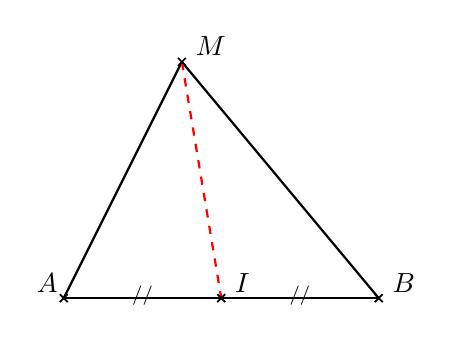
\begin{tikzpicture}[scale=1,>=stealth]

        % Définir les coordonnées des points A et B
        \coordinate (A) at (0,0);
        \coordinate (B) at (4,0);
        \coordinate (M) at (1.5,3);
        \coordinate (I) at (2,0);

        % Dessinez les vecteurs AB et AC
        \draw[thick,black] (A) -- (B) node[midway,anchor=south west] {};
        \draw[thick,black] (A) -- (M) node[midway,anchor=north west] {};
        \draw[thick,black] (M) -- (B) node[midway,anchor=north west] {};
        \draw[thick,red,dashed] (M) -- (I) node[midway,anchor=north west] {};

        % Ajouter des signes d'égalité pour les segments AI et IB
        \node at ($(0, 0.55)!0.5!(I)$)[anchor=north] {\scriptsize{//}};
        \node at ($(I)!0.5!(4, 0.55)$)[anchor=north] {\scriptsize{//}};

        % Marquer les points A, B et M avec des croix plus petites et plus épaisses
        \draw[line width=0.6pt] (A) ++(-0.05,-0.05) -- ++(0.1,0.1) (A) ++(-0.05,0.05) -- ++(0.1,-0.1) node[anchor=south east] {$A$};
        \draw[line width=0.6pt] (B) ++(-0.05,-0.05) -- ++(0.1,0.1) (B) ++(-0.05,0.05) -- ++(0.1,-0.1) node[anchor=south west] {$B$};
        \draw[line width=0.6pt] (M) ++(-0.05,-0.05) -- ++(0.1,0.1) (M) ++(-0.05,0.05) -- ++(0.1,-0.1) node[anchor=south west] {$M$};
        \draw[line width=0.6pt] (I) ++(-0.05,-0.05) -- ++(0.1,0.1) (I) ++(-0.05,0.05) -- ++(0.1,-0.1) node[anchor=south west] {$I$};
    \end{tikzpicture}
\end{minipage}
\hfill
\begin{minipage}{0.65\textwidth}
    \begin{mdframed}[style=definitionStyle]
        \textbf{Définition :} ~\\
        Dans un triangle, la médiane issue d'un sommet est le segment qui joint un sommet et le milieu du côté opposé.
    \end{mdframed}
    \begin{mdframed}[style=proprieteStyle]
        \textbf{Théorème de la médiane :} ~\\
        Soit $A$, $B$ deux points du plan et $I$ le milieu de $[AB]$. \\
        Pour tout point $M$ du plan, on a $\overrightarrow{MA}\pdt\overrightarrow{MB}=MI^2-\frac{AB^2}{4}$
    \end{mdframed}
\end{minipage}




\subsection*{2. Théorème d'Al Kashi}

\begin{minipage}{0.6\textwidth}
    \begin{mdframed}[style=proprieteStyle]
        \textbf{Théorème d'Al Kashi \emph{(ou théorème de Pythagore généralisé ou loi des cosinus)} :} ~\\
        Soit $ABC$ un triangle. On pose $BC=a$, $CA=b$ et $AB=c$. \\
        Alors :
        \vspace{-8pt}
        \begin{itemize}
            \item $a^2=b^2+c^2-2bc\times\cos{(\hat{A})}$
            \item $b^2=a^2+c^2-2ac\times\cos{(\hat{B})}$
            \item $c^2=a^2+b^2-2ab\times\cos{(\hat{C})}$
        \end{itemize}
    \end{mdframed}
\end{minipage}
\hfill
\begin{minipage}{0.35\textwidth}
    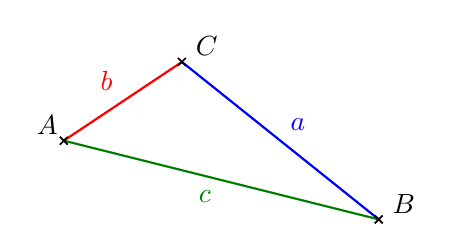
\begin{tikzpicture}[scale=1,>=stealth]

        % Définir les coordonnées des points A et B
        \coordinate (A) at (0,2);
        \coordinate (B) at (4,1);
        \coordinate (C) at (1.5,3);

        % Dessinez les vecteurs AB et AC
        \draw[dark_green, thick] (A) -- (B) node[midway,anchor=north east] {$c$};
        \draw[red, thick] (A) -- (C) node[midway,anchor=south east] {$b$};
        \draw[blue, thick] (C) -- (B) node[midway,anchor=south west] {$a$};

        % Marquer les points A, B et M avec des croix plus petites et plus épaisses
        \draw[line width=0.6pt] (A) ++(-0.05,-0.05) -- ++(0.1,0.1) (A) ++(-0.05,0.05) -- ++(0.1,-0.1) node[anchor=south east] {$A$};
        \draw[line width=0.6pt] (B) ++(-0.05,-0.05) -- ++(0.1,0.1) (B) ++(-0.05,0.05) -- ++(0.1,-0.1) node[anchor=south west] {$B$};
        \draw[line width=0.6pt] (C) ++(-0.05,-0.05) -- ++(0.1,0.1) (C) ++(-0.05,0.05) -- ++(0.1,-0.1) node[anchor=south west] {$C$};
    \end{tikzpicture}

\end{minipage}

\subsection*{3. Caractérisation du cercle}


\begin{minipage}{0.3\textwidth}
    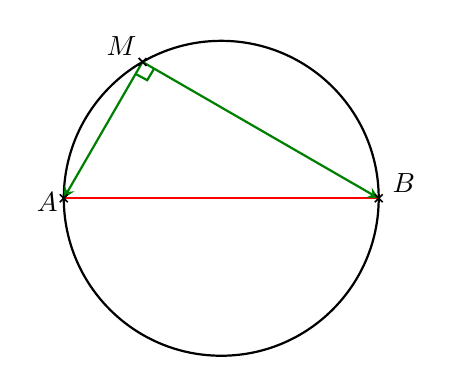
\begin{tikzpicture}[scale=1,>=stealth]

        % Définir les coordonnées des points A et B
        \coordinate (A) at (0,0);
        \coordinate (B) at (4,0);

        % Calculer le milieu du segment AB et le rayon du cercle
        \coordinate (M) at ($(A)!0.5!(B)$);
        \pgfmathsetmacro{\radius}{0.485*sqrt(17)}

        % Dessiner un arc de cercle pour représenter le lieu des points possibles pour le point C
        \draw[black, thick] (M) circle (\radius);

        % Choisir un angle pour positionner C sur l'arc de cercle
        \pgfmathsetmacro{\angle}{120}
        \coordinate (C) at ($(M)+(\angle:\radius)$);

        % Dessinez les vecteurs AB et AC
        \draw[red, thick] (A) -- (B) node[midway,anchor=north east] {};
        \draw[<-,dark_green, thick] (A) -- (C) node[midway,anchor=south east] {};
        \draw[->,dark_green, thick] (C) -- (B) node[midway,anchor=south west] {};

        % % Ajouter une marque d'angle droit en M
        \draw[dark_green, thick] (0.92, 1.575) -- (1.06, 1.5) -- (1.15, 1.65);

        % Marquer les points A, B et M avec des croix plus petites et plus épaisses
        \draw[line width=0.6pt] (A) ++(-0.05,-0.05) -- ++(0.1,0.1) (A) ++(-0.05,0.05) -- ++(0.1,-0.1) node[anchor=east] {$A$};
        \draw[line width=0.6pt] (B) ++(-0.05,-0.05) -- ++(0.1,0.1) (B) ++(-0.05,0.05) -- ++(0.1,-0.1) node[anchor=south west] {$B$};
        \draw[line width=0.6pt] (C) ++(-0.05,-0.05) -- ++(0.1,0.1) (C) ++(-0.05,0.05) -- ++(0.1,-0.1) node[anchor=south east] {$M$};
    \end{tikzpicture}
\end{minipage}
\hfill
\begin{minipage}{0.65\textwidth}
    \begin{mdframed}[style=proprieteStyle]
        \textbf{Propriété :} ~\\
        Soit $A$, $B$ et $M$ trois points du plan.
        $\overrightarrow{MA}\pdt\overrightarrow{MB}=0$ si et seulement si $M$ appartient au cercle de diamètre $[AB]$.
    \end{mdframed}

    \textbf{Remarque :} Cela revient à dire que l'ensemble des points $M$ tels que $\overrightarrow{MA}\pdt\overrightarrow{MB}=0$ est le cercle de diamètre $[AB]$. 
\end{minipage}

\text{ } ~\\ 

\textbf{Exemple :} ~\\
Soit $ABC$ un triangle tel que $AB=3$, $AC=4$ et $BC=5$ ($3$, $4$ et $5$ est appelé triplet pythagoricien car ils vérifie la relation de Pythagore : $3^2+4^2=5^2$). \\
\vspace{-8pt}
\begin{align*}
    \text{On a } 5^2  & = 3^2+4^2 \\
    \Leftrightarrow \text{ } BC^2 & = AB^2+AC^2 \text{ donc le triangle } ABC \text{ est rectangle en } A \text{.}
\end{align*}

Donc $\overrightarrow{AB}\pdt\overrightarrow{AC}=0$ donc $A$ appartient au cercle de diamètre $[BC]$.

\end{document}
% ----- FIN DU DOCUMENT -----